\documentclass[xcolor=pdftex,dvipsnames,table]{beamer}
\usecolortheme[accent=yellow,dark]{solarized}
\usepackage{etex}
\providecommand\thispdfpagelabel[1]{}
\usepackage{color}
\usepackage{xcolor}
\usepackage[latin1]{inputenc}
\usepackage[absolute,overlay]{textpos}
\usepackage{amsmath}
\usepackage{amssymb}
\usepackage{amsthm}
\usepackage{times}
\usepackage{listings}
\usepackage{graphics}
\usepackage{framed}
\usepackage{etex}
\usepackage[all]{xy}
\usepackage{xspace,listings,ulem,tikz}
\usepackage[outline]{contour}
\contourlength{1.2pt}
\usepackage[square,sort,comma,numbers]{natbib}
\usepackage{hhline}
\setbeamertemplate{footline}[frame number]
\tikzset{
    onslide/.code args={<#1>#2}{% http://tex.stackexchange.com/a/6155/16595
        \only<#1>{\pgfkeysalso{#2}}
    },
    hideshow/.style args={<#1><#2>#3}{%
        onslide=<#1>{move to},
        onslide=<#2>{#3}
    }
}

\lstset{
         basicstyle=\small\ttfamily, % Standardschrift
         %numbers=left,               % Ort der Zeilennummern
         numberstyle=\tiny,          % Stil der Zeilennummern
         %stepnumber=2,               % Abstand zwischen den Zeilennummern
         numbersep=5pt,              % Abstand der Nummern zum Text
         tabsize=2,                  % Groesse von Tabs
         extendedchars=true,         %
         breaklines=true,            % Zeilen werden Umgebrochen
         keywordstyle=\color{solarized@magenta},
         stringstyle=\color{solarized@yan}\ttfamily,
         identifierstyle=\color{solarized@blue},
         commentstyle=\color{solarized@base01},
         emphstyle=\color{solarized@red},
         showspaces=false,           % Leerzeichen anzeigen ?
         showtabs=false,             % Tabs anzeigen ?
         xleftmargin=3pt,
         framexleftmargin=3pt,
         framexrightmargin=1pt,
         framexbottommargin=3pt,
         language=C++,
         %backgroundcolor=\color{lightgray},
         showstringspaces=false,      % Leerzeichen in Strings anzeigen ?        
         escapeinside=||
 }
\lstset{
  emph={REAL, DYADIC, LAZY_BOOLEAN}
}
 \usetikzlibrary{arrows}
 \usepackage{caption}
\DeclareCaptionFont{white}{\color{white}}
\DeclareCaptionFormat{listing}{\colorbox[cmyk]{0.43, 0.35, 0.35,0.01}{\parbox{\textwidth}{\hspace{15pt}#1#2#3}}}
\captionsetup[lstlisting]{format=listing,labelfont=white,textfont=white, singlelinecheck=false, margin=0pt, font={bf,footnotesize}}
\beamertemplatenavigationsymbolsempty
\newcommand{\N}{\ensuremath{\mathbb{N}}} 
\newcommand{\R}{\ensuremath{\mathbb{R}}} 
\newcommand{\RR}{\ensuremath{\mathbb{R}}} 
\newcommand{\C}{\ensuremath{\mathbb{C}}} 
\newcommand{\Q}{\ensuremath{\mathbb{Q}}} 
\newcommand{\Z}{\ensuremath{\mathbb{Z}}} 
\newcommand{\D}{\ensuremath{\mathbb{D}}}
\newcommand{\lb}{\mathrm{lb}}
\newcommand{\dy}{\mathrm{dy}}
\newcommand{\cc}{\texttt{C++}\xspace}
\newcommand{\bin}{\mathrm{bin}}
\newcommand{\irram}{\texttt{iRRAM}\xspace}
\newcommand{\code}[1]{\texttt{#1}}
\newcommand{\sharpp}{\ensuremath{\#\mathcal P}\xspace}
\newcommand{\sharppu}{\ensuremath{\#{\mathcal P}_1}\xspace}
\newcommand{\fp}{\ensuremath{\mathcal{FP}}\xspace}
  \newcommand{\baana}{\code{BA\_ANA}\xspace}
  \newcommand{\anarect}{\code{ANA\_RECT}\xspace}
  \newcommand{\powerseries}{\code{POWERSERIES}\xspace}
  \newcommand{\poly}{\code{POLY}\xspace}
  \newcommand{\func}{\code{FUNC}\xspace}
  \newcommand{\real}{\code{REAL}\xspace}
  \newcommand{\complex}{\code{COMPLEX}\xspace}
  \newcommand{\temp}{\textcolor{red}}
  \newcommand{\seq}{\mathbf}
\newcommand{\fpu}{\ensuremath{\mathcal{FP}_1}\xspace}
\DeclareMathOperator{\dom}{\mathrm{dom}}
\newtheorem{conjecture}{Conjecture} 
\newtheorem{representation1}{Representation 1} 
\newtheorem{representation1b}{Representation 1'} 
\newtheorem{representation2}{Representation 2} 
\title[Analytic Continuation in iRRAM]{Analytic Continuation in \irram}
\author[A. Kawamura, F. Steinberg, H. Thies]{
		Akitoshi Kawamura, Florian Steinberg, Holger Thies 
}
\institute[JAIST]{
	Japan Institute of Science and Technology, Ishikawa Prefecture
}

\definecolor{solarized@base03}{HTML}{002B36}
\definecolor{solarized@base02}{HTML}{073642}
\definecolor{solarized@base01}{HTML}{586e75}
\definecolor{solarized@base00}{HTML}{657b83}
\definecolor{solarized@base0}{HTML}{839496}
\definecolor{solarized@base1}{HTML}{93a1a1}
\definecolor{solarized@base2}{HTML}{EEE8D5}
\definecolor{solarized@base3}{HTML}{FDF6E3}
\definecolor{solarized@yellow}{HTML}{B58900}
\definecolor{solarized@orange}{HTML}{CB4B16}
\definecolor{solarized@red}{HTML}{DC322F}
\definecolor{solarized@magenta}{HTML}{D33682}
\definecolor{solarized@violet}{HTML}{6C71C4}
\definecolor{solarized@blue}{HTML}{268BD2}
\definecolor{solarized@cyan}{HTML}{2AA198}
\definecolor{solarized@green}{HTML}{859900}
\begin{document}
\setbeamercolor{note}{fg=black,bg=lightgray} 
\date{July 21, 2015}
\frame{
\titlepage
}
\frame[<+->]{
\frametitle{Table of Contents}
\tableofcontents
}
\section{Introduction}
\subsection{Motivation}
\begin{frame}[<+->]
	\frametitle{Motivation}
	We want to apply and refine results from real complexity theory to develop 
efficient numerical algorithms with the following properties:
\begin{itemize}[<+->]
	\item full specification
	\item sound semantics
	\item correctness
	\item closure under composition
\end{itemize}

\end{frame}
\begin{frame}
	\frametitle{Algorithm Engineering}
	\centering
	\includegraphics[width=0.7\textwidth]{approach.png}
\end{frame}
\begin{frame}[<+->]
\frametitle{iRRAM}
\begin{itemize}[<+->]
\item iRRAM is a C++ framework for exact real computations
\item Ordinary C++ is extended by datatype REAL for computing with real numbers
\item Usual arithmetic operations are implemented for REAL
\item Other functions like abs, power, root, modulo, exp, log, sin, cos are also available
\end{itemize}
\end{frame}
\begin{frame}
  \frametitle{\irram: Real Number Representation}
  \centering
    \begin{tikzpicture}[remember picture, overlay]
     \node[font=\huge] at (0,0) {$x \in [\textcolor{green}{d}-\textcolor{red}{e},\textcolor{green}{d}+\textcolor{red}{e}]$};
     \draw<2-> [->, line width=3pt,color=green] (-1,0.4) -- (-1,2);
     \node<2->[color=green,font=\large] at (-1,2.2) {Multiple precision floating point number};
     \draw<3-> [->, line width=3pt,color=red] (2.4,-0.4) -- (2.4,-2);
     \node<3->[color=red,font=\large] at (2.4,-2.2) {$e = z \cdot 2^p$ (p,z \code{long})};
    \end{tikzpicture}
\end{frame}

\begin{frame}[<+->][fragile]
\frametitle{Example: \irram}
\begin{example}
\begin{lstlisting}
REAL series(int n){
  return power(REAL(2), -n);
}
REAL xinv_approx(long p, REAL& x){
  int N=-2*p+3;
  REAL ans = 0.0;
  for(int i=0; i<=N; i++)
    ans += series(i)*power(x,i);
  return ans;
}
REAL xinv(REAL& x) { return limit(xinv_approx, x);}
\end{lstlisting}
\end{example}
\end{frame}

\include{motivation}
\include{powerseries}
\include{implementation}
\begin{frame}

    \vspace{\fill}
\begin{beamercolorbox}[center,shadow=true,rounded=true]{note} 
        \huge Thank you!
\end{beamercolorbox}

    \vspace{\fill}
\end{frame} 
{
\makeatletter % to change template
    \setbeamertemplate{headline}[default] 
    \def\beamer@entrycode{\vspace*{-\headheight}} 
\makeatother
\begin{frame}{References}
\fontsize{6pt}{7.2}\selectfont 
\nocite{*}
\def\newblock{}
\bibliographystyle{abbrv}

\begin{thebibliography}{10}   

  \beamertemplatearticlebibitems
  \bibitem{6}
	Harvey Friedman,
    \newblock \emph{ The computational complexity of maximization and integration}, Adv. in Math. 53 (1984), no. 1, 80-98. MR 748898 (86c:03037)
  \beamertemplatearticlebibitems
  \bibitem{1}
	Akitoshi Kawamura, Norbert Th. M\"{u}ller, Carsten R\"{o}snick, and
Martin Ziegler
    \newblock \emph{Parameterized Uniform Complexity in Numerics:
from Smooth to Analytic, from NP-hard to Polytime}, pre-print (2012).

  \beamertemplatearticlebibitems
  \bibitem{7}
	Ker-I Ko,
    \newblock \emph{ Complexity theory of real functions}, Progress in Theoretical Computer Science, Birkh\"{a}user Boston Inc., Boston, MA, 1991.
MR 1137517 (93i:03057)

  \beamertemplatearticlebibitems
  \bibitem{8}
	Ker-I Ko,
    \newblock \emph{  On the Computational Complexity of Ordinary Differential Equations}, Information and Control 58(1-3): 157-194 (1983)


  \beamertemplatearticlebibitems
  \bibitem{2}
	Norbert Th. M\"{u}ller,
    \newblock \emph{ The \irram: Exact Real Arithmetic in C++}, Computability and Complexity in Analysis (2000) .

  \beamertemplatearticlebibitems
  \bibitem{Mul95}
	Norbert Th. M\"{u}ller,
    \newblock \emph{ Constructive aspects of analytic functions}, Computability
and Complexity in Analysis (Ker-I Ko and Klaus Weihrauch, eds.),
Informatik Berichte, vol. 190, FernUniversit\"{a}t Hagen, September
1995, CCA Workshop, Hagen, August 19-20, 1995, pp. 105-114.

  \beamertemplatearticlebibitems
  \bibitem{4}
	Norbert Th. M\"{u}ller,
    \newblock \emph{ Uniform Computational Complexity of Taylor Series}, ICALP 1987: 435-444

  \beamertemplatearticlebibitems
  \bibitem{5}
	Norbert Th. M\"{u}ller,
    \newblock \emph{ Polynomial Time Computation of Taylor Series}, Proc. 22 JAIIO - PANEL 1993

  \beamertemplatearticlebibitems
  \bibitem{9}
	Marian B. Pour-El and J. Ian Richards,
    \newblock \emph{ Computability in analysis
and physics}, Perspectives in Mathematical Logic, Springer-Verlag,
Berlin, 1989. MR 1005942 (90k:03062)
  \beamertemplatearticlebibitems
  \bibitem{11}
	Florian Steinberg,
    \newblock \emph{A type of Taylor series for the C++ library iRRAM for exact real arithmetic} (draft) last edited November 28, 2013
  \beamertemplatearticlebibitems
  \bibitem{10}
	Klaus Weihrauch,
    \newblock \emph{Computable analysis}, Texts in Theoretical Computer
Science. An EATCS Series, Springer-Verlag, Berlin, 2000, An
introduction. MR 1795407 (2002b:03129)

  \end{thebibliography}

\end{frame}
}
\end{document}
